\input format.tex

\usepackage{graphicx}
\graphicspath{{cores/}}

\usepackage{environ}
\usepackage{colortbl,array,booktabs}
\usepackage{tabularx}
\usepackage{arydshln}
\newcolumntype{K}[1]{>{\centering\arraybackslash}p{#1}}

\usepackage[nodisplayskipstretch]{setspace}

\colorlet{TablaBordeSuperior}{topcolor}
\colorlet{TablaBordeInferior}{topcolor}
\colorlet{TablaCentroSuperior}{blue!1}
\colorlet{TablaCentroInferior}{blue!20}
\colorlet{FuenteCabeceraTabla}{white}

\newcolumntype{M}[1]{>{\centering\arraybackslash}m{#1}}

\tcbset{rtab/.style={
freelance,
frame code={
 \path[top color=topcolor,bottom color=topcolor]
   ([yshift=-#1*(\baselineskip+2pt)]interior.north west) --
   ([yshift=-#1*(\baselineskip+2pt)]interior.north east) {[sharp corners]--
    ([yshift=3pt]interior.north east) --
    ([yshift=3pt]interior.north west)} -- cycle;

  },
interior code={},
 }
}

\newcommand\fuentecabecera[1]{\textcolor{black}{\textbf{#1}}}


\begin{document}

\vspace*{6mm}
%% 各章节
\setlength{\arrayrulewidth}{1pt}
\fontsize{9.3pt}{11pt}\selectfont
\color{gray2}

\begin{tctabularx}{tabularx={m{15.4cm}<{\centering}}}
\\[-6pt]
\cellcolor{topcolor} \raisebox{2.614pt}{\color{black70}\fontsize{11pt}{11pt}\selectfont\bf 健康建议}
\end{tctabularx}

\sepline

\vspace*{2mm}
\noindent
\tikz\draw[topcolor,fill=topcolor](0,0) rectangle(0.1,0.25);
{\fontsize{10pt}{11pt}\selectfont\bf {综合您本次肠道有益菌检测,您肠道健康保护力总得分为14.4分,
不利于肠道及人体健康,
建议您:}}

\noindent
\fontsize{8pt}{11pt}\selectfont
\arrayrulecolor{gray2}
\setlength{\arrayrulewidth}{.5pt}
\begin{center}
\begin{tabular}{|K{2.92cm}K{12.0cm}|}
\hline
\parbox[c][5.0cm]{.95\hsize}{
\noindent
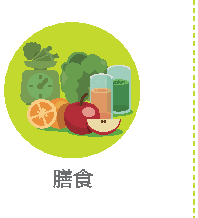
\includegraphics[scale=1.0]{baohulifoodwithvline.pdf}
}
 &
\hspace*{4mm}
\parbox{.95\hsize}{
\vspace*{3mm}
\begin{spacing}{1.5}

\includegraphics[scale=1.0]{xiaofangkuai.pdf}
{\fontsize{8pt}{11pt}\selectfont 保持良好的饮食结构。建议保持定时定量进餐的好习惯,早餐不可忽略。食物种类新鲜多样,交替食用。主食搭配适量粗粮,多食用各种新鲜的蔬菜水果,深绿色蔬菜至少占蔬菜总摄入量的一半。控制油炸类、西式快餐、含糖饮料等高脂高糖高热量食物。忌暴饮暴食。减少外出就餐的次数。戒烟限酒。}
\\

\includegraphics[scale=1.0]{xiaofangkuai.pdf}
{\fontsize{8pt}{11pt}\selectfont {建议适量多吃糙米、南瓜、橘子、四季豆、燕麦,这些食物能帮助栖粪杆菌属、阿克曼氏菌属、双歧杆菌属的增殖,有利于提高肠道保护力。}}
\end{spacing}
} \\
\hline

\parbox[c][5.0cm]{.95\hsize}{
\noindent

\includegraphics[scale=1.0]{baohuliprebioticswithvline.pdf}
}
 &
\hspace*{4mm}
\parbox{.95\hsize}{
\vspace*{3mm}
\begin{spacing}{1.5}

\includegraphics[scale=1.0]{xiaofangkuai.pdf}
{\fontsize{8pt}{11pt}\selectfont 建议适量补充益生元。您可选择补充菊粉、低聚果糖、富含多酚的蔓越莓提取物、豆类食物、低聚木糖等益生元,能帮助栖粪杆菌属、阿克曼氏菌属、双歧杆菌属在肠道内增殖,增加有益物质的产生,有利于增强肠道屏障功能,促进肠道健康。}
\\

\includegraphics[scale=1.0]{xiaofangkuai.pdf}
{\fontsize{8pt}{11pt}\selectfont 建议适量补充益生菌。您可选择补充含益生菌活菌饮料等益生菌产品,以增加您肠道内有益菌的含量,并能抑制有害菌的异常增殖,调节肠道菌群平衡。}
\end{spacing}
} \\
\hline
\parbox[c][5.0cm]{.95\hsize}{
\noindent

\includegraphics[scale=1.0]{baohuliprobioticswithvline.pdf}
}
 &
\hspace*{4mm}
\parbox{.95\hsize}{
\vspace*{3mm}
\begin{spacing}{1.5}

\includegraphics[scale=1.0]{xiaofangkuai.pdf}
{\fontsize{8pt}{11pt}\selectfont 日常注意戒烟限酒、避免熬夜、控制体重、保持愉快的情绪。}
\\

\includegraphics[scale=1.0]{xiaofangkuai.pdf}
{\fontsize{8pt}{11pt}\selectfont 建议您进行更详细的肠道菌群检测并持续监测,获取更具有针对性的膳食方案、微生态制剂推荐及运动指导等健康管理建议,为您的肠道健康保驾护航。}
\end{spacing}
} \\
\hline
\end{tabular}
\end{center}

{\noindent\qihao *温馨提示:以上健康建议仅供参考,您的实际膳食、运动及营养补充需根据您的自身具体情况进行调整。}
\vspace*{1cm}

\end{document}
